\subsection{Data pre-processing}
\label{S:DATAEDITINGPREPROCESSING}

Data pre-processing is a step taken ahead of data analysis.
In most cases, the set of available time series is heterogeneous because data is recorded from different systems of acquisition that are not synchronized with respect to time.
Therefore, the raw data do not usually share the same timestamp vectors.
This is an issue because BDLM is not capable to analyze asynchronous time series.
Therefore, the main objective of data pre-processing is to synchronize the time series. 
Moreover, data pre-processing includes time series selection, data analysis time period selection, \lstinline[basicstyle = \mlttfamily \small ]!NaN! removal, and data resampling.
%The time synchronization is performed automatically through the data editing process.

\begin{lstlisting}[ frame = single, basicstyle = \mlttfamily \scriptsize,  linewidth = \linewidth, caption = OpenBDLM data editing menu,  label = LST:Editing_menu, float = h!, ,captionpos=b]
- Data editing and preprocessing. Choose from:

     1  ->  Select time series
     2  ->  Select data analysis time period 
     3  ->  Remove missing data
     4  ->  Resample
     5  ->  Change synchronization options

     6  ->  Reset changes
     7  ->  Save changes and continue analysis

     choice >> 
\end{lstlisting}    

\subsubsection{Selection of time series}
\label{SS:SelectionTimeSeries}

The selection of time series allows including a subset of the time series. Note that time series are automatically synchronized as they are added to (or removed from) the dataset.

\subsubsection{Selection of data analysis time-window}
\label{SS:SelectionPeriodAnalysis}

The selection of the analysis time-window allows selecting a portion of data between two dates.
The date format follows \textquotesingle YYYY-DD-MM\textquotesingle {}.
If the second date entered exceeds the date associated with the last data sample of the original dataset, padding with \lstinline[basicstyle = \mlttfamily \small ]!NaN! values is performed. 
The timestep for the padding must be provided by the user.

\subsubsection{Removing missing data}
\label{SS:MissingDataRemoval}

It is possible to control the maximum amount of missing data (\lstinline[basicstyle = \mlttfamily \small ]!NaN!) allowed at each time slice. 
The maximum amount of \lstinline[basicstyle = \mlttfamily \small ]!NaN! allowed at each time slice is given in percent with respect to the total number of time series.
By default, the maximum amount of missing data is 100\% (see variable \lstinline[basicstyle = \mlttfamily \small ]!misc.options.NaNThreshold!).

\subsubsection{Data resampling}
\label{SS:DataResampling}
Data resampling changes the sampling rate of the time series according to a given timestep provided by the user. 
If the requested timestep is higher than the original data timestep, \lstinline[basicstyle = \mlttfamily \small ]!NaN! values are added.
Conversely, if the requested timestep is lower than the original  data timestep, OpenBDLM averages the data amplitude values within non-overlapping fixed time windows, each having the duration of the requested timestep.
The first time window starts at the first timestamp, and the new timestamps are assigned at the times corresponding to the mid point of each time window.

\subsubsection{Time synchronization options}
\label{SS:synchronization}
By default, the time synchronization in OpenBDLM is done by padding with \lstinline[basicstyle = \mlttfamily \small ]!NaN! values.
The time synchronization is controlled by the \lstinline[basicstyle = \mlttfamily \small ]!NaNThreshold! and \lstinline[basicstyle = \mlttfamily \small ]!tolerance! variables.
\lstinline[basicstyle = \mlttfamily \small ]!NaNThreshold!  is given in percent with respect to the total number of time series.
The variable \lstinline[basicstyle = \mlttfamily \small ]!tolerance! gives the duration (in number of days) after which two timestamps are not considered equal.
The default values for \lstinline[basicstyle = \mlttfamily \small ]!NaNThreshold!  and \lstinline[basicstyle = \mlttfamily \small ]!tolerance! are 100\% and $10^{-6}$ days, respectively (see variables \lstinline[basicstyle = \mlttfamily \small ]!misc.options.NaNThreshold! and \lstinline[basicstyle = \mlttfamily \small ]!misc.options.tolerance!). % $100$\% and $10^{-6}$ days, respectively. 

Figure \ref{FIG:time_sync} illustrates of how missing data removal, data-resampling and time synchronization are controlled by the parameters  \lstinline[basicstyle = \mlttfamily \small ]!misc.options.NaNThreshold! and \lstinline[basicstyle = \mlttfamily \small ]!misc.options.tolerance!.
\begin{figure}[htbp]
\begin{subfigure}{\linewidth}\centering
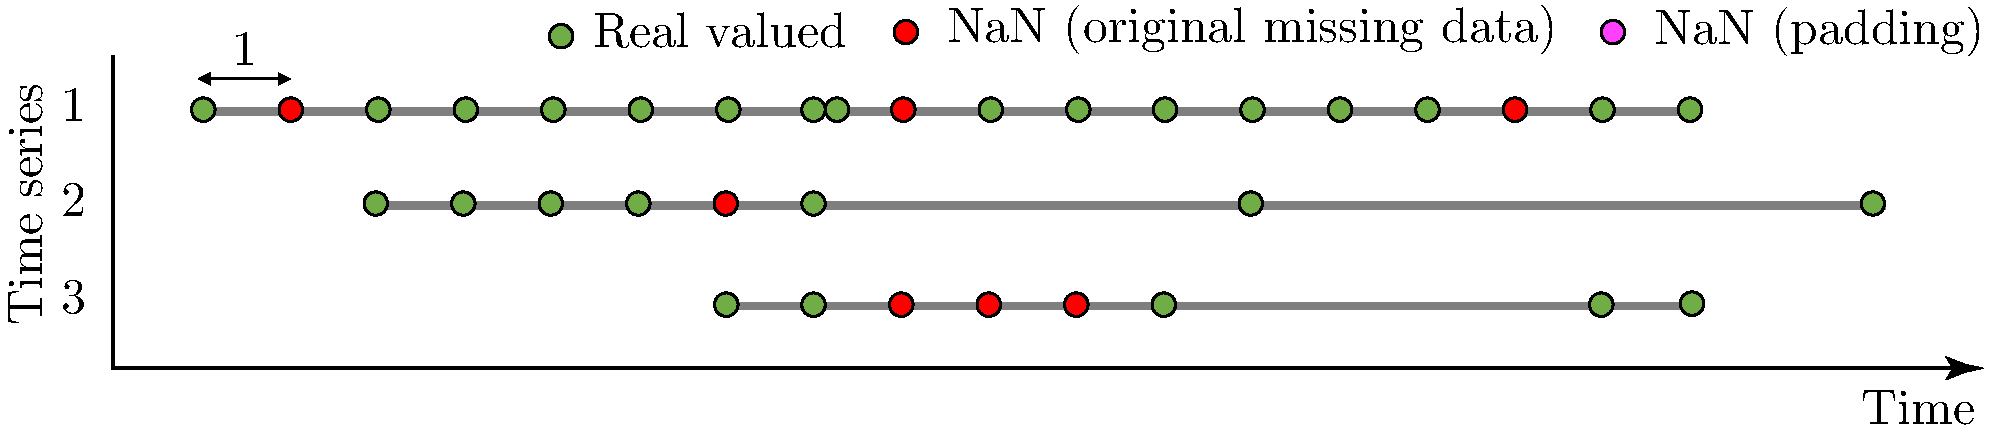
\includegraphics[width=0.9\linewidth]{./docfigs/time_synchro_1.pdf}\\[-8pt]
\caption{Original time series without modifications}
\end{subfigure}\\[12pt]
\begin{subfigure}{\linewidth}\centering
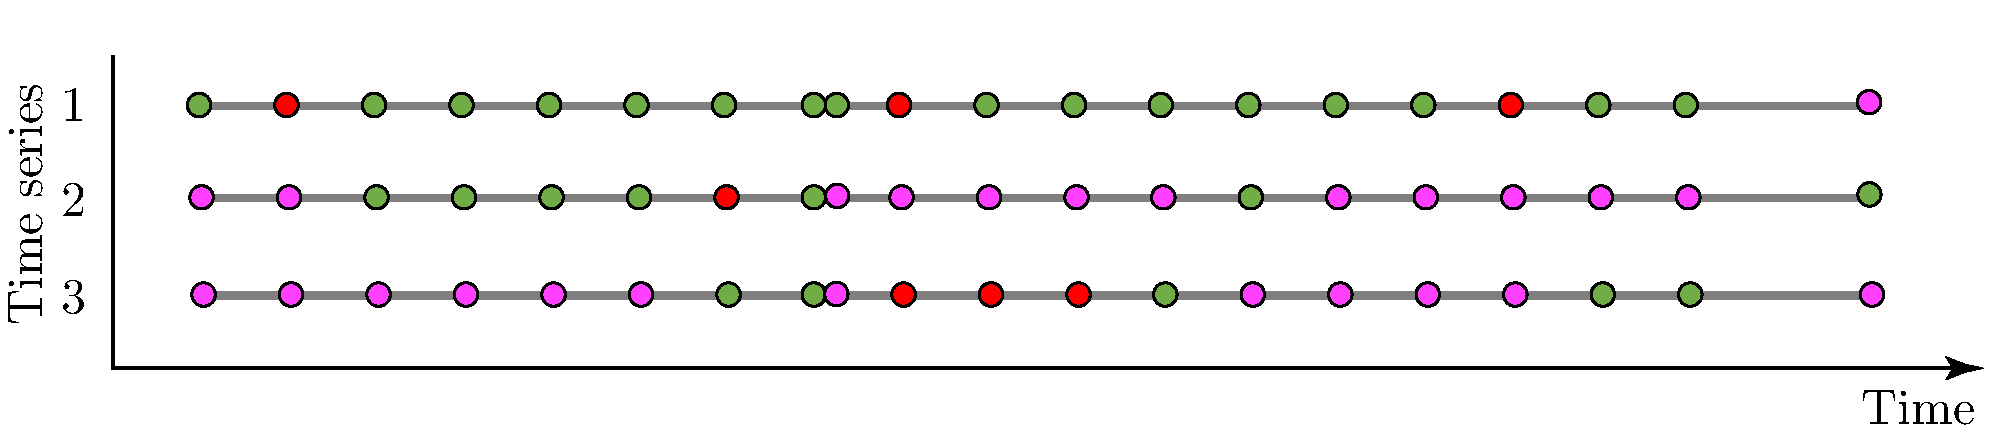
\includegraphics[width=0.9\linewidth]{./docfigs/time_synchro_2.pdf}\\[-8pt]
\caption{NaNThreshold$\,=100$\%, tolerance$\,=0.000001$}
\end{subfigure}\\[12pt]
\begin{subfigure}{\linewidth}\centering
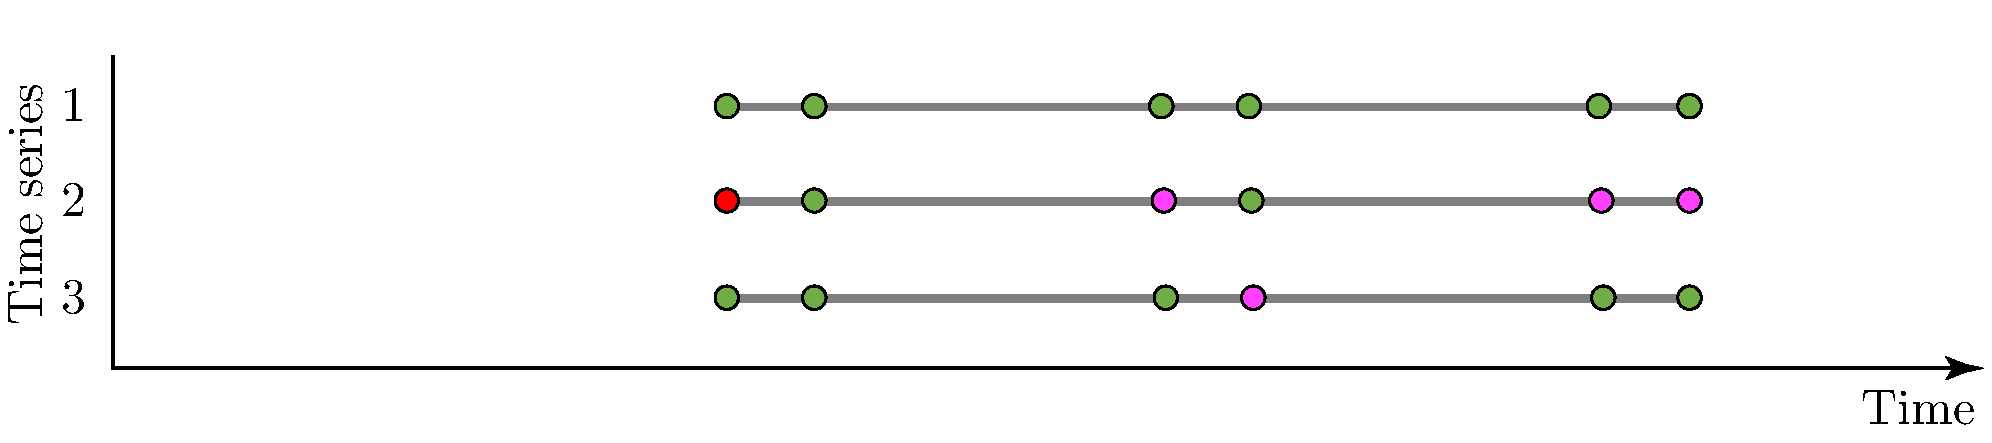
\includegraphics[width=0.9\linewidth]{./docfigs/time_synchro_3.pdf} \\[-8pt]
\caption{NaNThreshold$\,=50$\%, tolerance$\,=0.000001$}
\end{subfigure}\\[12pt]
\begin{subfigure}{\linewidth}\centering
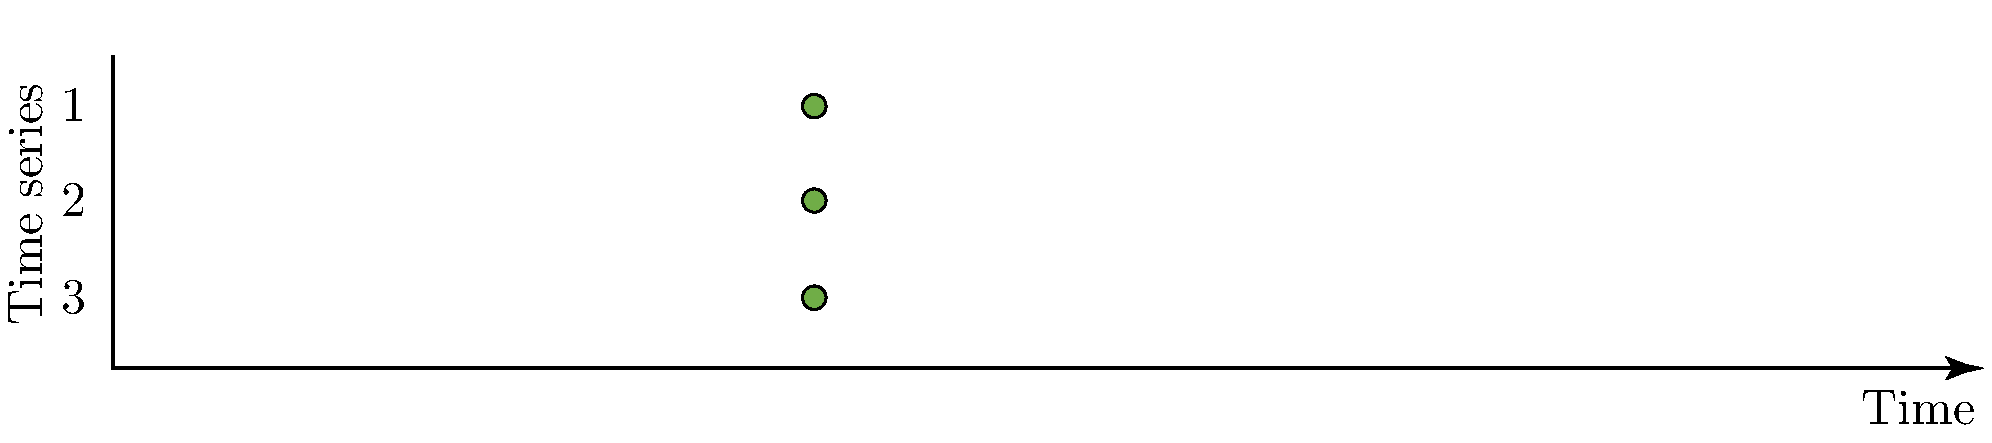
\includegraphics[width=0.9\linewidth]{./docfigs/time_synchro_4.pdf} \\[-8pt]
\caption{NaNThreshold$\,=0$\%, tolerance$\,=0.000001$}
\end{subfigure}\\[12pt]
\begin{subfigure}{\linewidth}\centering
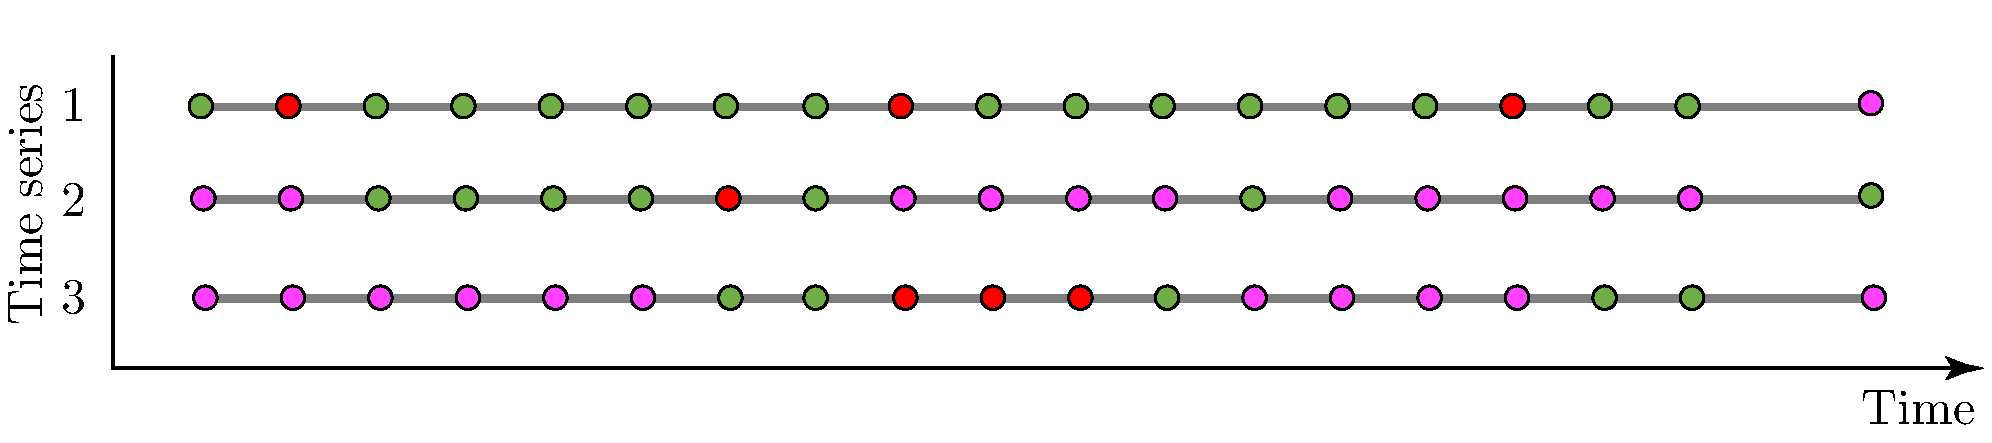
\includegraphics[width=0.9\linewidth]{./docfigs/time_synchro_5.pdf} \\[-8pt]
\caption{NaNThreshold$\,=100$\%, tolerance$\,=0.5$}
\end{subfigure}
\caption{Illustration of how missing data removal, data-resampling and time synchronization are controlled by the parameters  NaNThreshold and tolerance.}
\label{FIG:time_sync}
\end{figure}

\subsubsection{Data pre-processing functions}

The data pre-processing workflow is presented Figure~\ref{FIG:DataEditingWorkflow}. The list of OpenBDLM functions used for data editing is:

\begin{description}[style=unboxed]\setlength\itemsep{0em}
\item[Control script to pre-process the dataset (selection, resampling, etc..)] \leavevmode
  \begin{lstlisting}[ basicstyle = \mlttfamily \small, breaklines=true]
[data,misc,dataFilename]=editData(data,misc,varargin)
 \end{lstlisting}

\item[Requests the user to select some time series] \leavevmode
  \begin{lstlisting}[ basicstyle = \mlttfamily \small, breaklines=true]
[data,misc]=chooseTimeSeries(data,misc)
 \end{lstlisting} 
 
\item[Creates a single time vector from a set of time series] \leavevmode
  \begin{lstlisting}[ basicstyle = \mlttfamily \small, breaklines=true]
[data,misc]=mergeTimeStampVectors(dataOrig,misc,varargin)
 \end{lstlisting} 
 
\item[Resamples dataset according to a given timestep] \leavevmode
  \begin{lstlisting}[ basicstyle = \mlttfamily \small, breaklines=true]
[data_resample,misc]=resampleData(data,misc,varargin)
 \end{lstlisting} 
 
 \item[Selects data between two dates] \leavevmode
  \begin{lstlisting}[ basicstyle = \mlttfamily \small, breaklines=true]
[data,misc]=selectTimePeriod(data,misc)
 \end{lstlisting} 
 
  \item[Computes the timestep vector from the timestamps vector] \leavevmode
  \begin{lstlisting}[ basicstyle = \mlttfamily \small, breaklines=true]
[timesteps]=computeTimeSteps(timestamps)
 \end{lstlisting} 
 
   \item[Display information about stored data on screen] \leavevmode
  \begin{lstlisting}[ basicstyle = \mlttfamily \small, breaklines=true]
displayData(data,misc)
 \end{lstlisting} 
 
    \item[ Display the list of DATA\_*.mat files ] \leavevmode
  \begin{lstlisting}[ basicstyle = \mlttfamily \small, breaklines=true]
[FileInfo]= displayDataBinary(misc,varargin)
 \end{lstlisting} 
 
\end{description}

\begin{figure}[!h]
  \centering
  \captionsetup{justification=centering}
\scalebox{0.7}{
\begin{tikzpicture}

\node[paraamber](inputDataEditor){\lstinline[basicstyle = \mlttfamily \small ]!data!};
\node[esamber](editData)[below of = inputDataEditor,  yshift=-0.65cm, xshift = 0cm ]{ \phantom{} editData.m \phantom{} } ;
\node[esamber](editFunctions)[below of = editData, yshift = -1.25cm]{\begin{tabular}{c} chooseTimeSeries.m \\ selectTimePeriod.m \\ mergeTimeStampVectors.m \\ resampleData.m \end{tabular}};
\node[paraamber](DataMATFile)[below of =editFunctions, yshift=-1.75cm, xshift = 0cm]{\begin{tabular}{c} \lstinline[basicstyle = \mlttfamily \small ]!data.timestamps! \\ \lstinline[basicstyle = \mlttfamily \small ]!data.values! \\ \lstinline[basicstyle = \mlttfamily \small ]!data.labels! \\ \lstinline[basicstyle = \mlttfamily \small ]!DATA_*.MAT!  \end{tabular}};

\path[->, thick] (inputDataEditor)edge(editData);
\path[->, thick] (editData)edge(editFunctions);
\path[->, thick] (editFunctions)edge(DataMATFile);

\end{tikzpicture} } 
\caption{Data pre-processing workflow} \label{FIG:DataEditingWorkflow}
\end{figure}

